\documentclass[12pt]{tcc} 

\usepackage[brazil]{babel} 
\usepackage[T1]{fontenc}
%\usepackage[brazilian,hyperpageref]{backref}
\usepackage[hidelinks]{hyperref}
\usepackage[pt-BR]{datetime2}
\DTMlangsetup{showdayofmonth=false}
\usepackage[portuguese,ruled,linesnumbered,algochapter,titlenumbered]{algorithm2e}


% As figuras ficam armazenadas na pasta figuras
\graphicspath{{./figures/}}

% Informações do trabalho
\newcommand\dtitle{Framework para Análise de Desempenho de Consultas Web}
\newcommand\dauthor{Nome do Discente 1\\Nome do Discente 2}
\newcommand\dadvisor{Orientador, D.Sc.\\Coorientador}

% Definição de acronimos
\newacro{TCC}{Trabalho de Conclusão de Curso}
\newacro{GPT}{Transformador Pré-treinado Generativo}

\begin{document}
\pagenumbering{gobble}
\pagenumbering{roman}

\dcover

\dcoverback
	
\dlibrary{ficha.pdf}
		
\ddedicatory{
	\raggedleft \normalsize Dedicatória.
}

\dacknowledgment{
	Agradece-se à CAPES, CNPq e FAPERJ pelo financiamento parcial desta pesquisa.\\
	\\
	Agradece-se também Noname.
}

\dresumo{
Na web globalizada atual, a quantidade de dados gerados e consumidos pelas aplicações tem sido cada vez maior, e com isso existe uma importante preocupação com fatores performáticos.
Consumo de memória e escolha no formato dos arquivos para armazenamento se encontram dentro dessas preocupações no processo de P\&D de software atualmente.
Nesse contexto, existe uma demanda por ferramentas de medição, as quais sejam escaláveis, leves, e facilmente integráveis por desenvolvedores e pesquisadores para comparar diferentes opções de implementação em seus projetos, essas que impactam grandemente no resultado do trabalho.
Esse artigo propõe uma ferramenta Javascript para análise de performance no lado do cliente, que torna possível a pesquisadores e desenvolvedores testarem diferentes opções de implementação dentro de suas aplicações com a ajuda de outras pessoas executando esse código em seus aparelhos.
Dessa forma, a ferramenta também entrega ao desenvolvedor os dados dessas execuções estruturados, podendo ser integrado com frameworks de análise de dados.
}{palavras chaves separadas por ponto e vírgula}	

\dabstract{
	Resumo escrito em inglês
}{palavras chaves separadas por ponto e vírgula}

\dtables
	

\pagenumbering{arabic}
\justifying
	
\chapter{Introdução}
\label{sec:introducao}

Desde o começo da era da informação e principalmente com a popularização dos smartphones a quantidade de informações geradas por nós atingiu uma taxa de crescimento exponencial \citep{Gandomi2015Beyond}.
Este cenário com disponibilidade de grandes volumes de dados (do inglês, \emph{big data}), criou diversas oportunidades para modelos de negócios voltados para o uso desses dados.
Empresas como Google e Meta (antigo Facebook), se tornaram gigantes do mercado explorando estes modelos de negócios baseados em dados.

Entretanto, o manuseio de grandes volumes de dados necessita de cuidados especiais.
Pois, o volume dos dados podem superar os tamanhos de qualquer memória principal ou secundária as quais são encontradas no mercado.
Alguns exemplos desses tratamentos especiais para o manuseio de grandes volumes de dados são o modelo de programação MapReduce \citep{Dean2008MapReduce} e o sistema de armazenamento de objetos Haystack \citep{Beaver2010Finding}.
Portanto, os sistemas os quais manuseiam grandes volumes de dados precisam ser planejados para sua carga de trabalho.

Por outro lado, aplicações Web com arquitetura cliente-servidor sofrem com o problema da variedade de possíveis configurações tanto de hardware quanto de software no lado cliente.
Os desenvolvedores dessas aplicações muitas vezes não possuem uma ampla gama de ambientes para realizarem testes, o que pode levar a problemas em determinados tipos de ambientes.
Além disso, mesmo no caso onde existe acesso a diferentes tipos de ambiente, é improvável que a equipe de desenvolvimento tenha acesso direto, sendo necessário a colaboração de alguém externo ao desenvolvimento.

Por esses problemas, estamos propondo um framework o qual um desenvolvedor de qualquer aplicação Web seja capaz de facilmente obter métricas e estatísticas sobre provas de conceito as quais precisam ser executadas em diversas configurações de clientes por terceiros.
Por exemplo, considere uma aplicação Web a qual precisa trafegar um volume grande o suficiente de dados entre o cliente e o servidor, de modo que seja impossível de manter todos dados no cliente.
Para realizar o tráfego de dados, a equipe de desenvolvimento possui duas opções de formato de arquivo, utilizando arquivos CSV ou JSON.
Para tomar essa decisão, a equipe decide por criar provas de conceito e executá-las em diferentes tipos de cliente.
Porém, para que seja possível a execução por terceiros, além da prova de conceito a equipe ainda precisaria desenvolver como expor, como executar e como coletar as métricas.

Este é o tipo de cenário para qual o framework está sendo proposto, por disponibilizar uma aplicação Web casca para provas de conceito escritas nas linguagens JavaScript.
Além de sem a necessidade de adaptações no código, já seja capaz de coletar as métricas de execução da prova de conceito e informações do ambiente executando.
Deste modo, o desenvolvedor pode focar nas provas de conceito e na obtenção de ambientes e voluntários para seus testes, ao invés do desenvolvimento de um ambiente de testes.

Além disso, o trabalho está dividido em quatro capítulos.
O capítulo 2 e 3 correspondem aos aspectos metodológicos e trabalhos relacionados encontrados no campo de estudo.
O capítulo 4 apresenta a proposta de desenvolvimento da ferramenta.
Por fim, o capítulo 5 apresenta o estado atual do framework e o cronograma para a próxima etapa.


\chapter{Fundamentação teórica}
\label{sec:background}
	\label{sec:fund_teorica}

Para o levantamento da bibliografia foram utilizados: 
a ferramenta Elicit, um assistente de pesquisa baseado em um modelo \acr{GPT} de aprendizado de máquina.
E, a ferramenta Connected Papers, a qual para uma dada pesquisa gera um grafo de pesquisas similares baseado em cocitações e acoplamento bibliográfico.

A ferramenta Elicit funciona recebendo um string de busca, a qual pode ser uma pergunta em linguagem natural, para retornar uma página com as 7 pesquisas e um resumo das informações chave em um formato de tabela.
Portanto, no Elicit utilizei ao todo 15 strings de busca e consultei até a segunda página de resultados, totalizando 210 pesquisas encontradas, considerando duplicações.

\begin{table}[!ht]
	\centering
	\caption{Strings de busca utilizadas na ferramenta Elicit}
	\begin{tabular}{c L{1.5cm} R{1.5cm}}
		\toprule
		\textbf{String} \\
		\midrule
		``browsing memory'' \\
		``client side memory performance'' \\
		``client side memory profiling'' \\
		``memory network management web client'' \\
		``memory network performance web client'' \\
		``memory network profiling web client'' \\
		``memory network waste web client'' \\
		``measuring performance in client side'' \\
		``measuring in client side'' \\
		``performance measurement'' \\
		``tools to measure performance in client side'' \\
		``evaluating latency on client side'' \\
		``optimizing web browsing'' \\
		``performance tool web client side'' \\
		``waste resources client side'' \\
		``waste resources web client'' \\
		``web client side memory performance'' \\
		``What are the impacts of memory management in mobile Web Browsing?'' \\
		``What is the state-of-the-art for measuring performance of client side?'' \\
		``What is the state-of-the-art for measuring QoE and memory of Web Browsing?'' \\
		\bottomrule
	\end{tabular}
	\label{tab:string-busca-elicit}
\end{table}

Além disso, duas das pesquisas encontradas por meio do Elicit também foram utilizadas como strings de busca na ferramenta Connected Papers.
O Connected Papers retorna para uma dada pesquisa, um grafo com as 40 pesquisas mais similares encontradas por ele.
As quais podem também ser visualizadas em um formato de tabela e ordenadas pela similaridade.

\begin{table}[!ht]
	\centering
	\caption{Strings de busca utilizadas na ferramenta Connected Papers}
	\begin{tabular}{c L{1.5cm} R{1.5cm}}
		\toprule
		\textbf{String} \\
		\midrule
		``Measuring Web Latency and Rendering Performance: Method, Tools, and Longitudinal Dataset''  \\
		``MemInsight: platform-independent memory debugging for JavaScript''  \\
		``Obtaining in-context measurements of cellular network performance''  \\
		\bottomrule
	\end{tabular}
	\label{tab:string-busca-connected-papers}
\end{table}

Para selecionar as pesquisas dentre as encontradas por meio tanto do Elicit quanto do Connected Papers foi utilizado um critério inspirado em árvores de decisão.
Onde após a leitura do resumo da pesquisa, são respondidas até três perguntas sobre a pesquisa e caso as três respostas sejam sim, ele será selecionado para uma leitura completa.
Porém, caso a resposta da primeira ou segunda pergunta seja não, a pesquisa é descartada.

\begin{figure}[!ht]
	\centering
	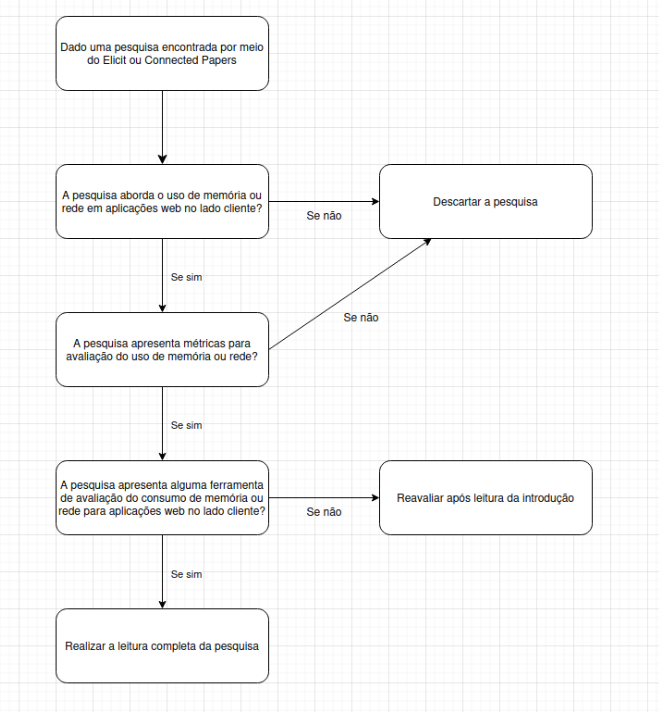
\includegraphics[width=0.6\textwidth]{figures/paper-decision-tree.png}
	\caption{Critérios utilizados para seleção de trabalhos para leitura.}
	\label{fig:fluxo-leitura}
\end{figure}

\begin{table}[!ht]
	\centering
	\caption{Trabalho Encontrados por Ferramenta}
	\begin{tabular}{c  c L{1.5cm} R{1.5cm}}
		\toprule
		\textbf{Ferramenta Utilizada} & \textbf{Quantidade} \\
		\midrule
		Elicit  &  280  \\
		Connected Papers  &  120  \\
		Total  &  400  \\
		Total Selecionados  &  15  \\
		\bottomrule
	\end{tabular}
	\label{tab:trabalhos-encontrados}
\end{table}

\chapter{Trabalhos Relacionados}
\label{sec:trabalhos_relacionados}
	\label{sec:trab_relacionados}

\begin{description}
	% \item \textbf{Paper 1}: Summary of the first paper goes here. This paragraph provides a concise overview of the paper's objectives, methodology, and key findings.

	\item[Jensen, 2015, MemInsight: Platform-Independent Memory Debugging for JavaScript:]
	Uma ferramenta criada por engenheiros da Samsung para gerar o perfil do consumo de memória de aplicações JavaScript.
	A ferramenta se diferencia por não se basear em snapshots, portanto, é capaz de obter o comportamento contínuo, por ser independente de plataforma e não precisa de uma engine de JavaScript modificada.
	
	\item[Arese, 2019, Measuring Web Latency and Rendering Performance: Method, Tools, and Longitudinal Dataset:]
	Apresenta a ferramenta Webget, uma ferramenta capaz de medir métricas de Web QoS como tempo de DNS, tempo até o primeiro byte e tempo de download. Além disso, ela também é capaz de capturar métricas de complexidade como quantidade e tamanho dos objetos do website.
	Cita a evolução da Web e o aumento da complexidade da tarefa de navegar pela Web. Algo que pode afetar consideravelmente a experiência do usuário (QoE), levando a consequências negativas para negócios. Além disso, este trabalho inclui um pouco de como a Web evoluiu e contém uma parte experimental robusta.

	\item[Bocchi, 2016, Measuring the Quality of Experience of Web users:]
	Aborda as métricas usadas para medir a qualidade de experiência dos usuários na Web. Dispondo o estado da arte, de 2016, das métricas e ferramentas, além de aplicá-las na Alexa top-100 páginas da Web e argumenta o impacto da QoE na receita das empresas, citando Big Techs.

	\item[Saverimoutou, 2020, Web View: A Measurement Platform for Depicting Web Browsing Performance and Delivery:]
	Propõem a plataforma automática Web View capaz de realizar medições em Website populares usando um ambiente de usuário representativo. Sua arquitetura é dividida em três partes: detectores, banco de dados e site de visualização. Sendo o objetivo da ferramenta realizar um monitoramento da QoE de um conjunto de sites.

	\item[Rajiullah, 2019, Web Experience in Mobile Networks: Lessons from Two Million Page Visits:]
	Tem como objetivo responder as perguntas:
	Quais são os principais fatores que afetam a navegação web em redes móveis?
	Quais os benefícios em usar novos protocolos como HTTP 2 e QUIC?
	Como os navegadores web impactam na QoE?
	Usa a plataforma aberta MONROE para realizar experimentos em redes móveis.

	\item[Qazi, 2020, Mobile Web Browsing Under Memory Pressure:]
	Uma investigação sobre o uso de memória dentro do contexto de navegação web. O artigo fala do aumenta da complexidade da navegação web, dando como evidências o aumento do tamanho médio de uma paǵina web em 6 vezes e como isso afeta o tempo de carregamento no ambiente mobile. Portanto, o artigo foca no aspecto do uso de memória e como isso impacta a navegação.

	\item[Naseer, 2021, WebMedic: Disentangling the Memory-Functionality Tension for the Next Billion Mobile Web Users:]
	Aborda os problemas de performance mais comuns na navegação web de usuários de países em desenvolvimento por usarem dispositivos low-end (baixo custo).

	\item[Gember, 2008, Obtaining in-context measurements of cellular network performancecript:]
	Provedores de internet, e também desenvolvedores, as vezes precisam entender como a internet móvel performa nos clientes. Essa medição é chamada in context, que significa a performance da internet somente quando o usuário está interagindo com a aplicação/aparelho. É dificil obter essa medição, devido a diversos fatores, como o contexto físico do aparelho, por exemplo.
	Esse paper fez um estudo sobre essa medição, utilizando dados de um provedor de internet e também de experimentos controlados, e desenvolveram um protótipo para Android de um medidor de performance para analisar a performance quando o dispositivo está ativo.
	O sistema consiste de um controller centralizado e aparelhos mobile rodando um serviço local para a medição. Administradores enviam requests para o controlador que contém as métricas de interesse, qual será o tempo da medição, ou outro requisito. Ex: medir latência nos Androids no Rio na hora do rush (18h). O controlador envia a requisição para os clientes que atendem os requisitos informados. Após a medição, os resultados são juntados e enviados para o admin pelo controlador.
	Esse medidor, pré instalado no dispositivo do cliente, recebe a requisição do controlador, e mandam inicialmente informações brutas para o controlador, como o consumo de internet , estado do dispositivo (se está com a tela ligada ou não) e outras informações do aparelho pra identificar quando é o momento de fazer a medição, e após isso começa propriamente a medição quando as condições são atendidas (o aparelho está ligado, está na hora informada, internet conectada). O serviço inicialmente coleta latência, throughput, streaming e o tempo de carregamento de páginas web, mas os autores dizem que é extensível. Não achei o nome da ferramenta, nem implementação.

	\item[Zhang, 2009, WPBench: a benchmark for evaluating the client-side performance of web 2.0 applications
	:]
	Propõe uma ferramenta chamada WPBench de benchmark para avaliar responsividade dos browsers/aplicações modernas. São removidas as variações de servidores e de redes para deixar mais parecido com o que o usuário interage. Ele grava as interações típicas do usuário com uma aplicação web, e depois reproduz em diversos browsers para fazer o benchmark. Eles conseguem manter as mesmas características de servidor, rede e as mesmas interações do usuário, gerando uma comparação mais justa.

	\item[Nikravesh, 2015, Mobilyzer: An Open Platform for Controllable Mobile Network Measurements:]
	No contexto de medição de rede, surgiu o Mobilyzer (Nikravesh, 2015), uma plataforma aberta para medição de rede em dispositívos móveis. Essa plataforma foi criada com o objetivo de prover uma solução escalável, eficiente e controlável, que fosse possível de ser incorporada tanto a apps em desenvolvimento, quanto em apps que já estão desenvolvidos, para suportar pesquisas e testes em medição de rede. 
	Ela funciona utilizando alguns componentes básicos, sendo eles:
	Uma biblioteca Android, que é integrada aos aplicativos para coletar as informações e enviar ao servidor. Ela é incorporada direto no código fonte.
	Um componente chamado Measurement Manager, no qual o pesquisador pode inserir medições de forma customizada e mais eficiente. Ele também realiza o scheduling das medições, e também cordena e monitora os dispositivos para que não tenha sobrecarga em nenhum aparelho ou rede medida.
	Um servidor em cloud, que fica responsável por coletar, analisar aplicando regras e publicar os dados coletados dos dispositivos. Essa arquitetura centralizada simplifica o compartilhamento de dados entre essas etapas, podendo integrar outras ferramentas de analise de dados com a base das coletas.
	Uma dificuldade no uso do Mobilyzer em pesquisas é que essa plataforma se restringe ao ambiente mobile, e apenas na plataforma Android. Isso restringe bastante possibilidades de medição em pesquisas multiplataforma. Nesse contexto, seria interessante trazer uma solução que contemplasse multiplas plataformas para essas medições.

	\item[Client-side performance profiling of JavaScript for web applications:]
	Essa tese descreve como foi criado um profiler genérico para JavaScript em aplicações web. Primeiramente, o desempenho do lado do cliente nas aplicações web é explicado e os fatores que contribuem para esse desempenho são discutidos. Para garantir que diferentes métodos possam ser comparados quantitativamente, foi desenvolvido um método de avaliação. Vários métodos foram propostos e avaliados antes da implementação do método de perfilamento. Para permitir uma fácil integração com qualquer aplicação web, foi criada uma ferramenta de integração. Embora o profiler tenha algum impacto no desempenho da aplicação, ele foi considerado preciso, fácil de usar e portátil.

	\item[Using a Proxy to Measure Client-Side Web Performance::]
	Apresentam o design e a implementação de um método para medir várias variáveis relacionadas à navegação do lado do cliente de páginas da web. Por exemplo com este método, é possivel medir a contribuição das consultas DNS para a latência total ao carregar uma página da web, conforme experimentada pelo usuário.

	\item[BenchLab: An Open Testbed for Realistic Benchmarking::]
	Apresenta uma ferramenta para fazer bachmark em aplicações web. Essa ferramenta testa as uma aplicação simulando um usuario usando a aplicação, usando aplicações geralmente usadas para testes como o Selenium.

	\item[Architectural Characterization of Client-side JavaScript Workloads \& Analysis of Software Optimizations:]
	O paper apresenta uma caracterização arquitetural detalhada de uma nova suíte de testes de referência para JavaScript, bem como uma análise de perfil do mecanismo de tempo de execução v8 JavaScript, popularmente utilizado pela Google. A análise ilustra o impacto arquitetônico de otimizações específicas do tempo de execução, bem como insights adicionais sobre a interação entre o mecanismo de tempo de execução e diferentes aplicações JavaScript. As avaliações são realizadas com versões de estoque de novas cargas de trabalho de JavaScript do lado do cliente do JetStream, bem como em versões modificadas que fecham a lacuna de representação em nível de programa com sites do mundo real.
utiliza várias ferramentas de benchmark focadas no javascript: SunSpider, Octane e JetStream.

	\item[JSMeter: Comparing the Behavior of JavaScript Benchmarks with Real Web Applications:]
	Neste artigo, é avaliado o comportamento do JavaScript em aplicações web comerciais e comparado com benchmarks, como SunSpider e V8. O estudo mediu dois aspectos específicos do tempo de execução do JavaScript: funções e códigos e eventos e manipuladores. Os resultados mostram que os benchmarks não são representativos de muitos sites reais e que as conclusões tiradas a partir deles podem ser enganosas. Alguns comportamentos comuns de sites reais, como a execução orientada a eventos, a predominância de códigos inativos e a prevalência de funções curtas, são subestimados nos benchmarks.

	
	\end{description}


\chapter{Método} 
	\label{sec:metodologia}

\section{Exemplo conceitual: Comparando o desempenho entre os formatos de arquivo JSON e CSV}

Imagine que você seja um pesquisador ou um desenvolvedor que decidiu utilizar a nossa ferramenta para sanar uma dúvida que encontrou ao desenvolver sua pesquisa:
O que possui melhor desempenho em um grande conjunto de dados? Transferir usando um arquivo CSV ou um arquivo JSON? A nossa ferramenta poderia ajudar.

Modelando o problema, o Projeto seria a sua aplicação, que seria composto por Tarefas, ou seja, a Tarefa é o que você realiza na sua aplicação e deseja realizar medições. Porém, podemos ter Tarefas simples, como no caso de uma medição única do tempo de download do arquivo, ou Tarefas Compostas, que poderia ser um pipeline completo de download e consulta utilizando um dos formatos de arquivo (realizar o download do arquivo, abrir no registro x dentro do arquivo, imprimir a informação). Ou seja, existe uma grande flexibilidade na elaboração de Tarefas.

A análise seria um conjunto de métricas. No nosso exemplo, algumas métricas possíveis são:

\begin{itemize}
	\item Tempo gasto.
	\item Largura de banda.
	\item Tamanho do arquivo.
	\item Informações do ambiente de execução.
	\item Gasto de memória.
\end{itemize}

Essas métricas, quando agrupadas, dão forma a uma análise, que representa uma medição utilizando um dos métodos a serem testados. No nosso exemplo, teríamos ao final do experimento duas análises: uma referente as medições acima utilizando o método CSV e outra utilizando o método JSON.

\section{Diagrama conceitual}

Na elaboração de qualquer projeto de software, a construção de um bom esquema conceitual é extremamente importante e fundamental para o sucesso do desenvolvimento. Na nossa ferramenta, possuímos algumas entidades principais. São elas:

\begin{figure}[!ht]
	\centering
	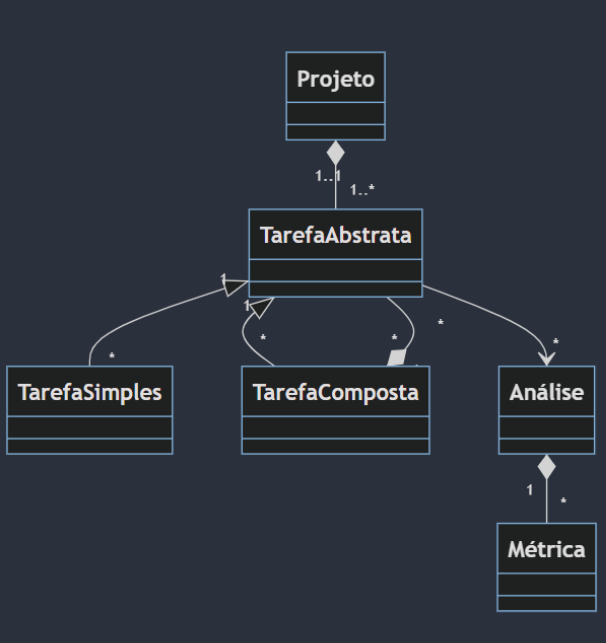
\includegraphics[width=0.6\textwidth]{figures/diagrama-conceitual.png}
	\caption{Diagrama conceitual}
	\label{fig:diag-conceitual}
\end{figure}

\begin{description}
	\item[Projeto:] Aplicação na qual o pesquisador está avaliando suas provas de conceito. É composto de uma lista de tarefas associadas, que constituem as ações que são executadas na aplicação e que desejam ser medidas pelo pesquisador/desenvolvedor. A cardinalidade da relação entre o Projeto e as Tarefas é de 1 para muitos, pois o Projeto deve ter pelo menos uma ou muitas Tarefas associadas a ele. 
	Ex: Projeto de construção de um transferidor de dados. Tarefas: fazer o download do arquivo, realizar a execução de um pipeline de consulta.
	
	\item[Tarefa Abstrata:] 
	Alguma ação executada no projeto com início, meio e fim. É representada por uma entidade abstrata, pois representa conceitualmente o que precisa ser executado no projeto. Pode ser descrita também como um roteiro de um processo ou procedimento sob avaliação. Essas ações podem ser fornecidas pelo pesquisador, ou pode ser parametrizada inicialmente pela ferramenta.

	\item[Tarefa Composta:] 
	Representa um conjunto de tarefas. Ex: Realização de um pipeline de consulta no arquivo (Tarefas agregadas: Realizar o download do arquivo, abrir o arquivo na linha X, realizar leitura).
	Utilizamos nessa entidade o padrão de software Composite, que nos permite representar facilmente um agrupamento de uma entidade. Nesse caso, a entidade folha seria uma Tarefa Simples, e o agrupamento a Tarefa Composta. Realizamos essa escolha pois simplifica a execução de múltiplas tarefas ao mesmo tempo, no caso de ser executado um pipeline grande de tarefas.

	\item[Análise:] 
	Um conjunto de métricas coletadas da execução de uma tarefa utilizando um método. Essas métricas correspondem aos dados desejados pelo pesquisador, e uma análise deve possuir uma ou mais métricas.
	Dessa forma, a saída das execuções das tarefas é uma análise, composta pelas métricas desejadas pelo pesquisador, e que se relaciona a Tarefa Abstrata. Uma Tarefa Abstrata pode estar relacionada a uma ou mais análises, e as análises podem estar relacionadas a uma ou mais tarefas, visto que é um agrupamento de métricas. Diferentes métodos gerarão diferentes análises, cada uma com as suas métricas.
	Ex: Uma Análise dos métodos de transferência de dados seria composta por: um cojunto de métricas, qual tarefa ela representa, e qual método ela está representando. Nesse caso teríamos duas análises, uma com o método JSON e uma com o método CSV.

	\item[Métrica:] 
	Uma medida quantitativa de algum recurso computacional do cliente. Ou seja, a unidade mais granular do sistema. Pode ser fornecida pela ferramenta ou inserida pelo pesquisador. Ex: O conjunto de métricas da Análise dos métodos de transferência de dados seria composto por: velocidade de transferência, tamanho do arquivo, tempo total de transferência, taxa de compressão do arquivo, entre outras.

\end{description}


\section{Diagrama de Classes}

Após a elaboração do diagrama conceitual, foi elaborado o Diagrama de Classes à seguir que dará base a implementação do sistema: 

O diagrama começa com a entidade Project, que representa um projeto, e que possui um método que executa todas as tarefas associadas a ele.
Além disso, um detalhe importante nessa entidade é o relacionamento com ExecutionProfile, que seria qual cliente está executando aquele projeto. Temos também que o Project pode possuir um ou mais IPersister, que é o método abstrato que representa os repositórios que realizarão as interações com as bases de dados. Em IPersister, podemos ter diversas instâncias.
No diagrama foi criada somente a SheetsonPersister, que será a nossa escolha inicial para base de dados.

Em seguida, vemos a classe abstrata Task, que representa as tarefas abstratas.
Ela possui o método público run(), que será como essa tarefa será executada, e os métodos privados execute(), preTaskJob() e postTaskJob(), que serão implementados pelas classes concretas.
Eles representam, respectivamente, a execução detalhada da tarefa, um conjunto de operações a serem realizadas antes da execução, e um conjunto de atividades a serem realizadas depois da execução da tarefa.

Após isso, temos a classe abstrata Metric, ou Métrica.
Nela temos os métodos públicos collect() e get(), que serão as interações externas com as métricas.
Temos também o método privado preProcessing(), que serve para realizar, se necessário, algum pré-processamento antes da coleta da métrica.
Temos dois exemplos de implementações concretas dessa classe no diagrama, são eles:
ProcessMemoryMetric e DeltaTimeMetric. O exemplo DeltaTimeMetric possui uma necessidade de pré-processamento, já que a variação de tempo é calculada com base em dois parâmetros diferentes, o que justifica a implementação desse método.


\begin{figure}[!ht]
	\centering
	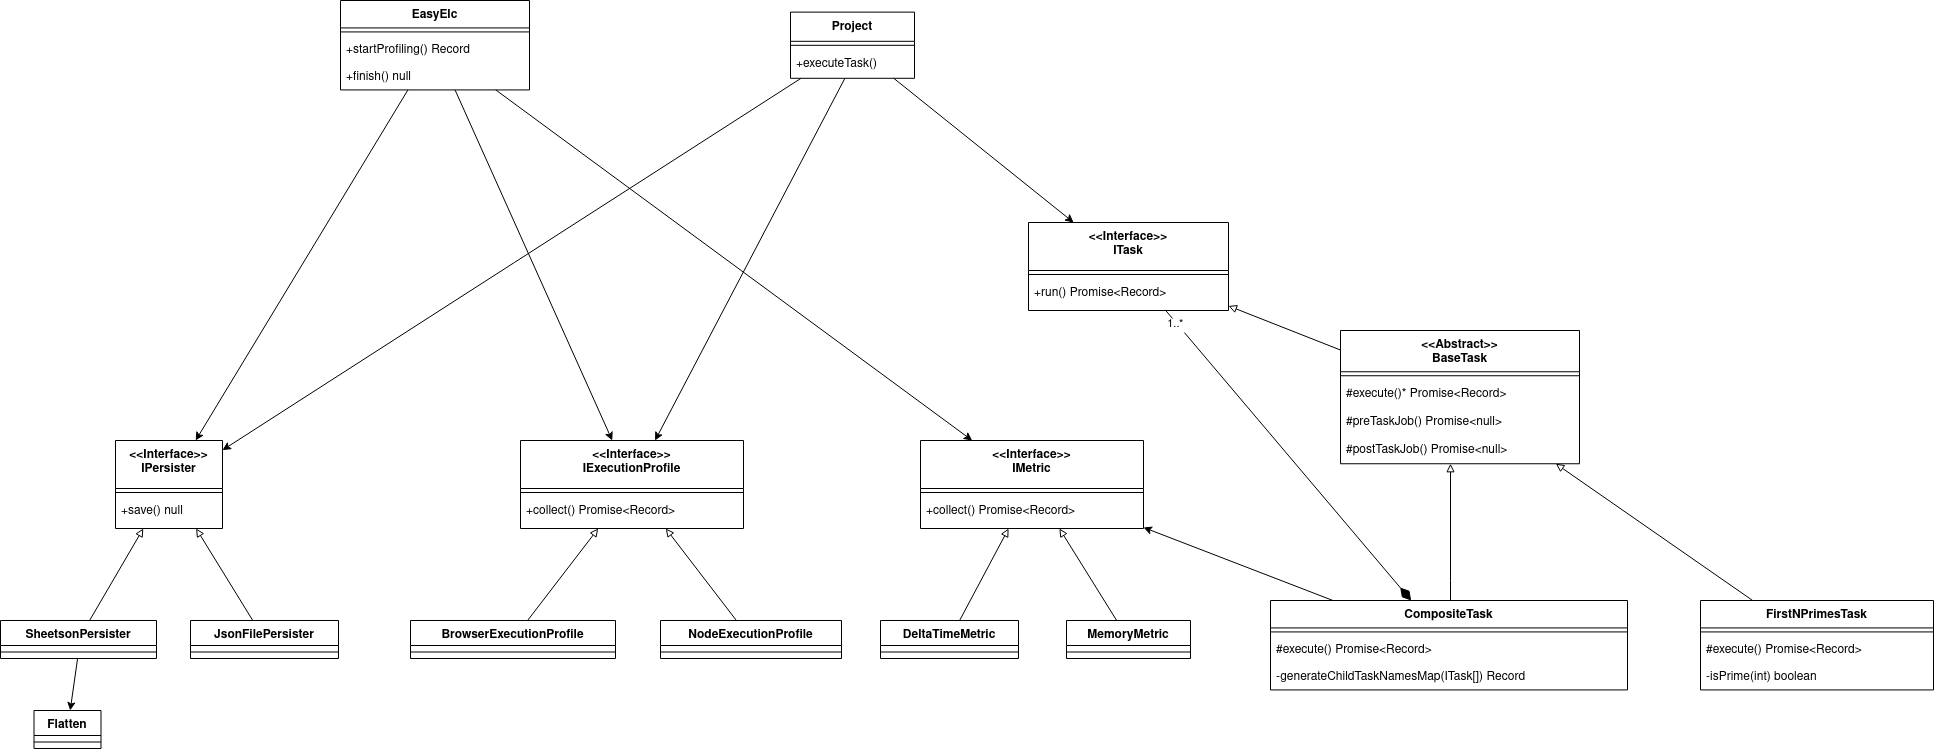
\includegraphics[width=0.6\textwidth]{figures/diagrama-classes.png}
	\caption{Diagrama classes}
	\label{fig:diag-classes}
\end{figure}


\section{Arquitetura}

Na utilização da aplicação, o pesquisador deve ser capaz de inserir suas métricas, suas análises, e chamar no código dele os métodos de coleta. Dessa forma, precisamos construir um ambiente no qual ele consiga realizar essas tarefas. Isso pode ser feito de diferentes formas, uma delas chamamos de abordagem tradicional, e a outra que propomos é utilizando a ferramenta Sheetson.

\subsection{Abordagem tradicional}

Nessa abordagem seria realizada a implementação de dois componentes principais: 

\begin{description}
	\item[Biblioteca Javascript:] Esse componente diz respeito a biblioteca que o pesquisador inserirá no código da sua aplicação, inserindo nela as métricas desejadas para medição.

	\item[Backend na núvem:] Esse componente receberia as requisições enviadas pela aplicação e condensaria em um banco de dados qualquer essas medições. Após isso, seria necessário o desenvolvimento de um front-end, para o pesquisador conseguir baixar esses arquivos.
\end{description}

Essa abordagem seria a mais comum, dado que possui similaridades com grande parte das aplicações que vemos hoje. Porém, essa implementação deixaria a aplicação com uma alta complexidade de uso, e além disso, não seria escalável, pois o backend precisa de adaptações para lidar com, por exemplo, múltiplos bancos de dados.
Nesse contexto, encontramos uma solução que se demonstrou interessante para o nosso problema.

\subsection{Sheetson}

O Sheetson é uma ferramenta gratuita, a qual torna possível a inserção e interação com uma planilha do Google Docs via API. Então a solução baseada nessa ferramenta seria:

\begin{description}
	\item[Biblioteca Javascript:] Esse componente diz respeito a biblioteca que o pesquisador inserirá no código da sua aplicação, inserindo nela as métricas desejadas para medição.
	
	\item[Sheetson:] O Sheetson receberia os dados enviados do cliente, e inseriria em uma tabela CSV, para download futuro.

\end{description}

Essa abordagem possui diversas vantagens, como poder isolar no desenvolvimento da biblioteca a classe que controlará a persistência dos dados, e implementar inicialmente utilizando o sheetson. Se quisermos posteriormente implementar a primeira abordagem e substituir por chamadas a um backend real, com qualquer base de dados que seja, seria necessário somente substituir essa implementação, porém hoje ganharíamos um tempo grande no desenvolvimento do projeto.

Além disso, o pesquisador poderia utilizar sua própria conta do Google para realizar suas pesquisas, eliminando a necessidade de contratar provedores de cloud ou de fazer deploy de alguma aplicação. Isso gera uma redução grande na complexidade do uso do projeto.


\chapter{Resultados}
\label{sec:aval_exp}

A avaliação experimental compreende uma avaliação quantitativa ou qualitativa do trabalho a partir de critérios estabelecidos para comparação. Como em qualquer experimento, a capacidade de reprodução é fundamental para sua validade. Sendo assim, é importante descrever o processo de experimentação adotados, apresentar os resultados propriamente dito, com uma síntese explicativa dos principais resultados. Finalmente, devem ser apresentadas as ameaças ao estudo, \emph{i.e.}, qualquer coisa que possa tirar ou limitar a validade do experimento conduzido. 

\chapter{Conclusão}
	\label{sec:conclusao}

	A conclusão é a finalização do trabalho e indica as conclusões obtidas com o desenvolvimento do trabalho, sejam elas positivas ou negativas. Nas conclusões, analisa-se o que era desejado (definido na introdução com os objetivos), comparando com o que foi alcançado pelo trabalho, descrevendo como os objetivos foram alcançados e o porquê de algum objetivo não ter sido alcançado. Destacam-se também as contribuições do trabalho, incluindo os benefícios e inovações trazidas pelo trabalho.

Apresentam-se os pontos do trabalho que merecem um maior aprofundamento de estudos. Isso possibilita a criação de novos trabalhos com estudos nesses pontos apresentados, na forma de uma continuidade das pesquisas efetuadas pelo trabalho. Os trabalhos futuros indicam, ainda, uma maturidade de pesquisa do autor do trabalho e esses pontos podem ser trabalhados, posteriormente.

\label{bibpage}
\renewcommand\bibname{Referências}
\addcontentsline{toc}{section}{Referências}
\bibliography{references}
%\bibliographystyle{plainnat}
\bibliographystyle{apalike}
\label{bibfinalpage}

\label{lastpage}
\end{document}